\chapter{Dead ends -de}

	Suppose that you know that some fact does not appear in any precondition nor delete effect of any action; also the fact is not in init nor goal. Then there are two possibilities, either it has the function that the action adding the fact may be used at most once (the action has another effect); or it is dead end (it is redundant). Such dead end facts can be removed together with actions that produce them.
	
	This operation does precisely this thing; it removes such redundant facts and actions
	
	\begin{figure}
		\begin{subfigure}[b]{0.4\textwidth}
			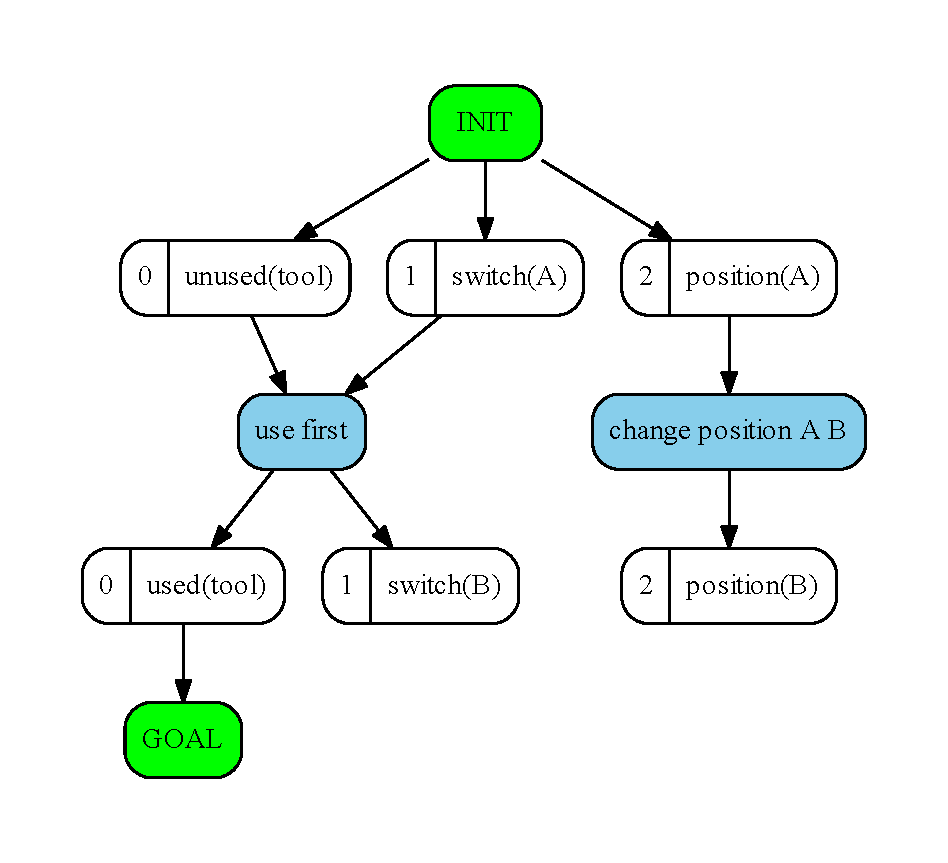
\includegraphics[scale=0.35]{deadEnds/figures/oneDeadEnd_input}
			\caption{before reduction}
		\end{subfigure}	
		\begin{subfigure}[b]{0.4\textwidth}
			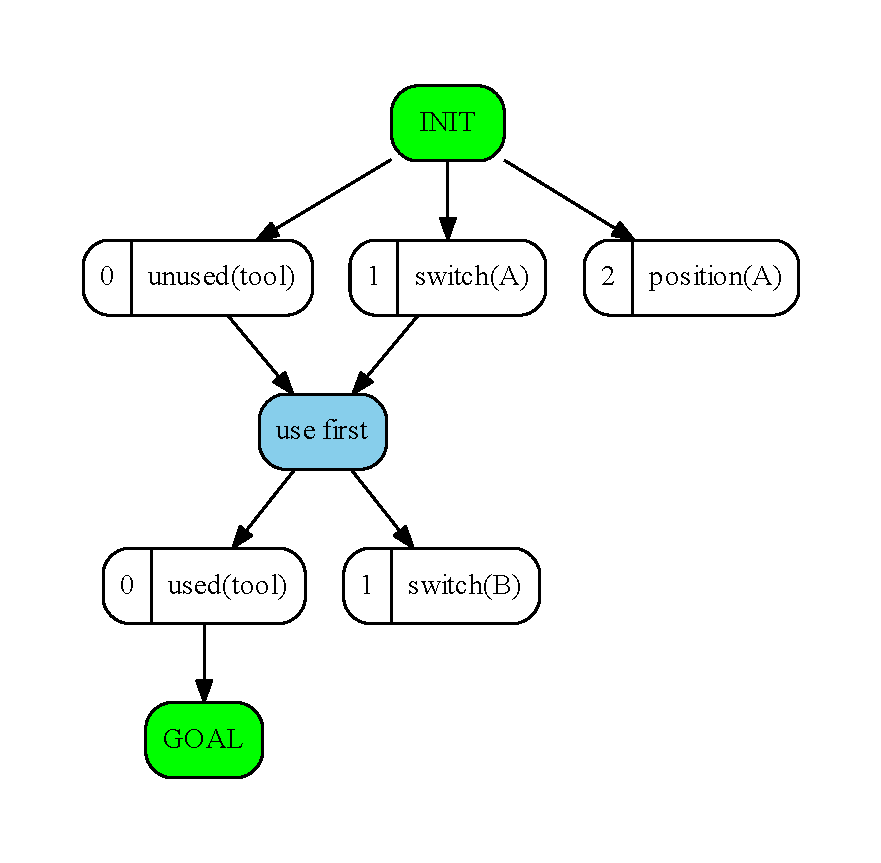
\includegraphics[scale=0.35]{deadEnds/figures/oneDeadEnd_output}
			\caption{after reduction}
		\end{subfigure}
		\caption{In this example fact \emph{2 position(A)} and action \emph{change position A B} may be removed because they are redundant. But fact \emph{switch(B)} cannot be removed because action \emph{use first} has more than one effect. }
	\end{figure}

	
	\section{Reduce operation}
	Let's have SAS in form $<\vars, \init, \goal, \actions, \mutexes{}>$. If there is a value $u$ such that:
	
	\begin{enumerate}
		\item $u \notin \init, u \notin \goal$
		\item $|\con{u}| =  0$
		\item there is no effect of type $<-1,u_i>, u_i \in \dom{\var{u}}$ in any $\actions{}$
		\item each action adding $u$ has only one effect; $1 = |\eff{a}| \forall a \in \pro{u}$	\label{de:in:invariants}
	\end{enumerate}

	Condition \ref{de:in:invariants} ensures that invariant won't be destroyed. If such condition would not be met, then delete relaxation could rise.

	Then the operation is executed. The operation does following things:
	
	\begin{enumerate}
		\item remove $u$ from domain of $\var{u}$
		\item remove $u$ from mutexes
		\item remove actions with zero effects
	\end{enumerate}
	
	Output of the reduction is SAS $<\vars{}', \init{}, \goal{}, \actions{}', \mutexes{}'>$.
	
	
	\section{Possible outgoing states of SAS}
	\begin{enumerate}
		\item possible empty mutex
		\item possible state of SAS for application DV
	\end{enumerate}

	\section{States before application of this operation}
	\begin{itemize}
		\item SAS from the beginning
		\item does not know any operation that could cause such state, so what about running dv only once to save time?
	\end{itemize}

	
	\section{Reverse operation}
	The reverse operation adds removed values and actions. No extending of plan is done.
	
	\section{Implementation notes}
	The operation is implemented in the way that it iteratively remove dead ends (values and actions) from the SAS untill there are any. Because by removing an value, actions that add that value are redundant and so on.
	
	
	
	